%===============================================================================
% LaTeX sjabloon voor de bachelorproef toegepaste informatica aan HOGENT
% Meer info op https://github.com/HoGentTIN/bachproef-latex-sjabloon
%===============================================================================

\documentclass{bachproef-tin}

\usepackage{hogent-thesis-titlepage} % Titelpagina conform aan HOGENT huisstijl
\usepackage{listings}
\usepackage{xcolor}

\definecolor{codegreen}{rgb}{0,0.6,0}
\definecolor{codegray}{rgb}{0.5,0.5,0.5}
\definecolor{codepurple}{rgb}{0.58,0,0.82}

\lstdefinestyle{codeStyle}{  
    belowcaptionskip=1\baselineskip,
    breaklines=true,
    frame=none,
    numbers=none, 
    basicstyle=\footnotesize\ttfamily,
    keywordstyle=\bfseries\color{green!40!black},
    commentstyle=\itshape\color{purple!40!black},
    identifierstyle=\color{blue},
    backgroundcolor=\color{gray!10!white},
}

\lstset{style=codeStyle}

\lstdefinelanguage{JavaScript}{
  keywords={break, case, catch, continue, debugger, default, delete, do, else, false, finally, for, function, if, in, instanceof, new, null, return, switch, this, throw, true, try, typeof, var, void, while, with},
  morecomment=[l]{//},
  morecomment=[s]{/*}{*/},
  morestring=[b]',
  morestring=[b]",
  ndkeywords={class, export, boolean, throw, implements, import, this},
  keywordstyle=\color{blue}\bfseries,
  ndkeywordstyle=\color{darkgray}\bfseries,
  identifierstyle=\color{black},
  commentstyle=\color{purple}\ttfamily,
  stringstyle=\color{red}\ttfamily,
  sensitive=true
}



%%---------- Documenteigenschappen ---------------------------------------------
% TODO: Vul dit aan met je eigen info:

% De titel van het rapport/bachelorproef
\title{Titel}

% Je eigen naam
\author{Steven Stevens}

% De naam van je promotor (lector van de opleiding)
\promotor{Jan Janssens}

% De naam van je co-promotor. Als je promotor ook je opdrachtgever is en je
% dus ook inhoudelijk begeleidt (en enkel dan!), mag je dit leeg laten.
\copromotor{Piet Pieters}

% Indien je bachelorproef in opdracht van/in samenwerking met een bedrijf of
% externe organisatie geschreven is, geef je hier de naam. Zoniet laat je dit
% zoals het is.
\instelling{---}

% Academiejaar
\academiejaar{2020-2021}

% Examenperiode
%  - 1e semester = 1e examenperiode => 1
%  - 2e semester = 2e examenperiode => 2
%  - tweede zit  = 3e examenperiode => 3
\examenperiode{1}

%===============================================================================
% Inhoud document
%===============================================================================

\begin{document}

%---------- Taalselectie -------------------------------------------------------
% Als je je bachelorproef in het Engels schrijft, haal dan onderstaande regel
% uit commentaar. Let op: de tekst op de voorkaft blijft in het Nederlands, en
% dat is ook de bedoeling!

% \selectlanguage{english}

%---------- Titelblad ----------------------------------------------------------
\inserttitlepage

%---------- Samenvatting, voorwoord --------------------------------------------
\usechapterimagefalse
%%=============================================================================
%% Voorwoord
%%=============================================================================

\chapter*{\IfLanguageName{dutch}{Woord vooraf}{Preface}}
\label{ch:voorwoord}

%% TODO:
%% Het voorwoord is het enige deel van de bachelorproef waar je vanuit je
%% eigen standpunt (``ik-vorm'') mag schrijven. Je kan hier bv. motiveren
%% waarom jij het onderwerp wil bespreken.
%% Vergeet ook niet te bedanken wie je geholpen/gesteund/... heeft

Deze bachelorproef werd geschreven in functie van het afronden van de opleiding Toegepaste Informatica aan de Hogeschool van Gent. Ook al volg ik de afstudeerrichting mobiele applicaties, waar webapplicaties een deel van zijn, toch is de module bundler nooit aan bod gekomen. Hoewel velen erop vertrouwen, weten weinigen wat ze voor essentiële taken verrichten. Door deze proef hoop ik dat er meer wordt stilgestaan bij het kiezen van een module bundler. 

Ik wil graag mijn promotor, Heidi Roobrouck, bedanken om deze scriptie in goede banen te leiden. Ook mijn co-promotor, Cedric Vanhaeverbeke, verdient een dankwoordje. Ik kon steeds rekenen op zijn uitgebreide feedback. Deze twee personen hebben ervoor gezorgd dat dit onderzoek tot een goed einde is gekomen.

%%=============================================================================
%% Samenvatting
%%=============================================================================

% TODO: De "abstract" of samenvatting is een kernachtige (~ 1 blz. voor een
% thesis) synthese van het document.
%
% Deze aspecten moeten zeker aan bod komen:
% - Context: waarom is dit werk belangrijk?
% - Nood: waarom moest dit onderzocht worden?
% - Taak: wat heb je precies gedaan?
% - Object: wat staat in dit document geschreven?
% - Resultaat: wat was het resultaat?
% - Conclusie: wat is/zijn de belangrijkste conclusie(s)?
% - Perspectief: blijven er nog vragen open die in de toekomst nog kunnen
%    onderzocht worden? Wat is een mogelijk vervolg voor jouw onderzoek?
%
% LET OP! Een samenvatting is GEEN voorwoord!

%%---------- Nederlandse samenvatting -----------------------------------------
%
% TODO: Als je je bachelorproef in het Engels schrijft, moet je eerst een
% Nederlandse samenvatting invoegen. Haal daarvoor onderstaande code uit
% commentaar.
% Wie zijn bachelorproef in het Nederlands schrijft, kan dit negeren, de inhoud
% wordt niet in het document ingevoegd.

\IfLanguageName{english}{%
\selectlanguage{dutch}
\chapter*{Samenvatting}
\lipsum[1-4]
\selectlanguage{english}
}{}

%%---------- Samenvatting -----------------------------------------------------
% De samenvatting in de hoofdtaal van het document

\chapter*{\IfLanguageName{dutch}{Samenvatting}{Abstract}}
Een module bundler of build tool is een essentieel onderdeel in het maken van moderne webapplicaties. Al jaren wordt Webpack gezien als de beste keuze hiervoor. Aangezien er genoeg andere opties zijn, vele met een nieuwe aanpak, is het wel eens tijd om die bewering nog eens na te gaan. In een literatuurstudie wordt de geschiedenis en werking van een module bundler geschetst. Daarna, aan de hand van een vergelijkende studie, worden drie populaire alternatieven tegenover Webpack geplaatst in rechtstreeks duel. Eerst wordt een nieuw project opgezet met de respectievelijke kandidaten. Daarna trachten we drie open-source projecten, elk met zijn eigen moeilijkheden, om te vormen van Webpack naar een tegenkandidaat. Doorheen dit gedocumenteerd proces, wordt er meer uitleg gegeven over de verschillende technologieën die aan bod komen. Tot slot wordt in de conclusie, rekening houdend met verschillende ob- en subjectieve factoren, de titel van deze proef beantwoord. 


%---------- Inhoudstafel -------------------------------------------------------
\pagestyle{empty} % Geen hoofding
\tableofcontents  % Voeg de inhoudstafel toe
\cleardoublepage  % Zorg dat volgende hoofstuk op een oneven pagina begint
\pagestyle{fancy} % Zet hoofding opnieuw aan

%---------- Lijst figuren, afkortingen, ... ------------------------------------

% Indien gewenst kan je hier een lijst van figuren/tabellen opgeven. Geef in
% dat geval je figuren/tabellen altijd een korte beschrijving:
%
%  \caption[korte beschrijving]{uitgebreide beschrijving}
%
% De korte beschrijving wordt gebruikt voor deze lijst, de uitgebreide staat bij
% de figuur of tabel zelf.

\listoffigures
\listoftables

% Als je een lijst van afkortingen of termen wil toevoegen, dan hoort die
% hier thuis. Gebruik bijvoorbeeld de ``glossaries'' package.
% https://www.overleaf.com/learn/latex/Glossaries

%---------- Kern ---------------------------------------------------------------

% De eerste hoofdstukken van een bachelorproef zijn meestal een inleiding op
% het onderwerp, literatuurstudie en verantwoording methodologie.
% Aarzel niet om een meer beschrijvende titel aan deze hoofstukken te geven of
% om bijvoorbeeld de inleiding en/of stand van zaken over meerdere hoofdstukken
% te verspreiden!

\chapter{\IfLanguageName{dutch}{Inleiding}{Introduction}}
\label{ch:inleiding}

De wijze waarop een webapplicatie gemaakt wordt, verandert continu. Het lijkt wel of er elke week een nieuw framework uitkomt met een iets andere aanpak dan al degene die hem voorgingen. Eén ding echter blijft al enkele jaren hetzelfde: de nood aan een module bundler is er nog steeds, voor nu toch.

Dit onderzoek tracht de noodzaak, werking en toekomst van de module bundler te schetsen. Dit aan de hand van een paar veel voorkomende implementaties ervan. Het uiteindelijke doel is om te bepalen of de huidige koning van de module bundlers, Webpack, nog steeds het recht heeft om die positie op te eisen.

\section{\IfLanguageName{dutch}{Probleemstelling}{Problem Statement}}
\label{sec:probleemstelling}

Dit onderzoek is in de eerste plaats gericht naar mijn co-promotor. Als webdeveloper komt hij vaak voor de keuze van welke module bundler te gebruiken. In de toekomst kan hij die beslissing dus maken aan de hand van deze vergelijkende studie. Daarnaast kan dit onderzoek ook een meerwaarde bieden voor andere webdevelopers, inclusief mezelf.

\section{\IfLanguageName{dutch}{Onderzoeksvraag}{Research question}}
\label{sec:onderzoeksvraag}

De hoofdonderzoeksvraag werd al eerder aangehaald: is het nog steeds gewettigd dan Webpack de meest gebruikte module bundler is?

\section{\IfLanguageName{dutch}{Onderzoeksdoelstelling}{Research objective}}
\label{sec:onderzoeksdoelstelling}

Hoewel de onderzoeksvraag beantwoorden aan de hand van een vergelijkende studie uiteraard het uiteindelijke doel is, hoop ik dat dit werk volgend doel ook verwezenlijkt.

De module bundler is voor velen, mijn co-promotor en mezelf erbij gerekend, iets wat ze gebruiken en nodig hebben maar niet zoveel over nadenken en weten. Vele frameworks om webapplicaties te maken komen met een module bundler ingebouwd. Zo wordt de keuze dus voor je gemaakt. Ideaal voor iemand die zich daar geen zorgen over wil maken maar aangezien de webapplicatie niet werkt zonder, is het de moeite om toch meer te weten erover. Het tweede, meer verborgen doel is dus om de module bundler en zijn werking te ontrafelen.

\section{\IfLanguageName{dutch}{Opzet van deze bachelorproef}{Structure of this bachelor thesis}}
\label{sec:opzet-bachelorproef}

% Het is gebruikelijk aan het einde van de inleiding een overzicht te
% geven van de opbouw van de rest van de tekst. Deze sectie bevat al een aanzet
% die je kan aanvullen/aanpassen in functie van je eigen tekst.

De rest van deze bachelorproef is als volgt opgebouwd:

In Hoofdstuk~\ref{ch:stand-van-zaken} wordt een overzicht gegeven van de stand van zaken binnen het onderzoeksdomein, op basis van een literatuurstudie.

In Hoofdstuk~\ref{ch:methodologie} wordt de methodologie toegelicht en worden de gebruikte onderzoekstechnieken besproken om een antwoord te kunnen formuleren op de onderzoeksvragen.

% TODO: Vul hier aan voor je eigen hoofstukken, één of twee zinnen per hoofdstuk

In Hoofdstuk~\ref{ch:conclusie}, tenslotte, wordt de conclusie gegeven en een antwoord geformuleerd op de onderzoeksvragen. Daarbij wordt ook een aanzet gegeven voor toekomstig onderzoek binnen dit domein.


\chapter{Stand van zaken}
\label{ch:stand-van-zaken}

Een moderne website wordt gemaakt met drie belangrijke technologieën: \gls{HTML} voor inhoud, \gls{CSS} voor vormgeving, en \gls{Javascript} om de pagina interactief te maken. Deze drie kunnen allemaal aan elkaar worden gekoppeld, ergens op een server worden gezet om vervolgens een werkende website te kunnen inladen. Ook al zijn de grote web platformen van vandaag, zoals Facebook en Youtube, allemaal gebaseerd op deze technologieën, zijn er veel meer ingrediënten nodig om ze te laten werken.

Voor het maken van een simpele, statische site zijn de drie basis technologieën
 van het web alles wat we nodig hebben. Het is echter een heel ander verhaal voor een ontwikkelaar die een complexere site wil maken, een reactieve site, een site die gebruik maakt van \gls{open-source} \gls{packages} of die gewoon zijn eigen werk wat makkelijker wil maken. Er zijn duizenden bibliotheken, \gls{packages} en frameworks die webontwikkeling mogelijk maken op een heel ander niveau en eenvoudiger dan ooit tevoren \autocite{npm-no-date}. Dit stelt ons echter voor een nieuw probleem. 

Als we een webapplicatie zouden maken met een enkel \gls{Javascript} bestand zonder afhankelijkheden i.e. geen andere bestanden die gelinkt zijn aan dat \gls{Javascript} bestand, het linken aan een index.html en tot slot wat \gls{CSS} toevoegen, zou die site prima werken. Maar wat als we een tweede \gls{Javascript} bestand introduceren en daar naar verwijzen in het andere bestand. Wat als we een \gls{open-source} package willen installeren en gebruiken, gedownload van een \gls{package-manager} zoals NPM? Wat als we \gls{SASS} willen gebruiken om \gls{CSS} uit te breiden? Dit zou allemaal niet werken. De browser weet gewoon niet hoe alle verschillende stukjes aan elkaar te plakken.
We hebben iets nodig dat alle verschillende  bestanden en zijn afhankelijkheden bundelt, iets dat de \gls{SASS} bestanden begrijpt en correct laadt, of welk ander bestand dan ook. We hebben een module bundler nodig. In essentie nemen zij alle verschillende bronbestanden in een project en bundelt die tot een enkel uitvoer bestand dat de browser begrijpt.

\section{Geschiedenis}

Om de rest van dit hoofdstuk te begrijpen, moet eerst de \gls{Javascript} module uitgelegd worden. Modulair programmeren splitst een programma op in brokken gebaseerd op functionaliteit en vaak in aparte bestanden. Deze brokken worden modules genoemd. Modules worden dan aan elkaar gekoppeld om een applicatie te vormen. \autocite{webpack-no-dateB} \autocite{mozilla-2021A}

Node.js, een runtime voor computers en servers waardoor \gls{Javascript} applicaties los van een browser kunnen draaien, ondersteunde modulair programmeren vanaf het begin met CommonJS. Ondersteuning voor modules in de browser daarentegen was niet bestaand. De eerste module bundlers kwamen pas na 2014. Om te begrijpen waarom ze bestaan, moeten we eerst weten hoe webapplicaties voor hen werden gebouwd en welk probleem ze oplosten. \autocite{webpack-no-dateA}

\subsection{Script tags}

\gls{Javascript} kan worden gekoppeld aan, of direct worden geschreven in, het \gls{HTML}-bestand van een site met behulp van script-tags \autocite{mozilla-2021}. Dit wetende, zouden we een verschillende tag en corresponderend \gls{Javascript} bestand kunnen gebruiken voor elke toepassing van de applicatie. Laten we zeggen dat er een bestand is met alle code voor het aanmelden van een gebruiker en een ander voor algemene gebeurtenissen (op een knop klikken, \ldots). Dit is prima wanneer we slechts twee bestanden hebben die niet zo groot zijn, maar introduceert knelpunten voor het dataverkeer wanneer dit geschaald zou worden naar een grotere applicatie \autocite{webpack-no-dateB}. Hetzelfde geldt als al de code in één groot bestand zou staan. Het globale domein van de browser zou ook vervuild raken met onze eigen functies. Aangezien sommige, of alle, functies beschikbaar zijn in het globale domein, zou dit veiligheidsrisico's en naam botsingen kunnen introduceren. 

\lstinputlisting[language=HTML]{codeSnippets/scriptTags.html}

\subsection{Immediately invoked function expressions}

Een Immediately invoked function expression of IIFE is een functie die wordt uitgevoerd zodra hij is gedefinieerd \autocite{mozilla-2021B}. Omdat elke IIFE een lokaal domein declareert, lossen ze het probleem van vervuiling van het globale domein op. De garbage collector van Javascript zorgt hiervoor \autocite{mozilla-2021C}. Het gebruik van IFFE’s heeft geleid tot zogenaamde task runners: ze voegen al de project bestanden samen. Het grote nadeel van task runners is dat wanneer één bestand wordt gewijzigd, het hele project opnieuw moet worden opgebouwd. Ook moeten alle afhankelijkheden zoals \gls{packages} van tevoren handmatig gedefinieerd worden. Ze maken het makkelijker om functies en hele scripts te hergebruiken, maar doen niets voor de build output te verkleinen. Je kunt nog steeds eindigen met een zeer groot \gls{Javascript} bestand dat de gebruiker moet downloaden. 

\lstinputlisting[language=Javascript]{codeSnippets/IIFE.js}

\subsection{CommonJS}

Vóór 2009 draaide \gls{Javascript} alleen in een browser \autocite{wikipedia-no-date}. Node.js introduceerde een \gls{Javascript} runtime die op computers en servers kon draaien. Dit bracht een nieuwe reeks uitdagingen met zich mee \autocite{crutchfield-2018}. Aangezien \gls{Javascript} niet in de browser draaide en er dus geen \gls{HTML} script-tags waren, hoe konden deze toepassingen nieuwe stukken code laden? 

CommonJS introduceerde de require functie \autocite{nodejs-2021}. Hiermee kan alles dat een externe module exporteert, worden geïmporteerd. Herbruikbare code kan nu worden geïmporteerd uit elk ander \gls{Javascript} bestand in een project. Het maakt het implementeren van dependency management eenvoudig te begrijpen.

Dit alles kwam met een groot addertje onder het gras: Het werkte, en werkt nog steeds, voor Node.js applicaties maar het is geen officiële functie van \gls{Javascript} en daarom ondersteunen browsers het niet \autocite{crutchfield-2018}. Omdat CommonJS de code niet bundelt, kunnen webbrowsers niet overweg met de verschillende geïmporteerde en geëxporteerde modules. Iets moet dat voor hen doen. 

\lstinputlisting[language=Javascript]{codeSnippets/commonJSExport.js}

\lstinputlisting[language=Javascript]{codeSnippets/commonJSImport.js}

\subsection{ECMAScript Modules}

CommonJS was geen officiële functie van Javascript. ECMAscript (=Javascript) heeft in versie 6 wel een eigen modulesysteem ingevoerd \autocite{orendorff-2015}. ECMAScript Modules of ESM, bereiken dezelfde doelen als CommonJS, maar met een andere syntax. Moderne browsers kunnen nu applicaties draaien die opgebouwd zijn met ES Modules \autocite{mozilla-2021}. Met de nadruk op moderne browsers.

\lstinputlisting[language=Javascript]{codeSnippets/esmExport.js}

\lstinputlisting[language=Javascript]{codeSnippets/esmImport.js}

\section{Module bundlers}

Ontwikkelaars zijn altijd op zoek naar manieren om hun leven gemakkelijker te maken. Ze willen om het even welk type van module, CommonJS of ESM, of om het even welk ander bestand (een afbeelding bijvoorbeeld) in hun project importeren en het in een kleiner uitvoerbestand naar de eindgebruiker verzenden. Zo werd de module bundler geboren.

De meest essentiële functie van een module bundler is het bijhouden van alle modules die geïmporteerd worden in een project, los van uit hoeveel bestanden het bestaat, en deze te bundelen in een enkel bestand genaamd de bundel. Die bundel wordt ook geminificeerd om zo klein mogelijk te zijn, zonder de functionaliteit aan te tasten. Ze doen dit door commentaar, witruimtes, nieuwe regels, ... te verwijderen. Ook worden variabele namen zo kort mogelijk afgekort. Al dit resulteert in een kleiner bestand.

Ongebundeld bestand: 147 bytes
\lstinputlisting[language=Javascript]{codeSnippets/unbundled.js}
Gebundeld bestand: 77 bytes
\lstinputlisting[language=Javascript]{codeSnippets/bundled.js}

Alle module bundlers van vandaag delen deze functies samen met gemeenschappelijke concepten. We zullen kijken naar de 2 belangrijkste. 

\subsubsection{Tree shaking}

Tree shaking is het proces van het verwijderen van ‘dead code’ \autocite{webpack-no-dateC}. Wanneer een module wordt geïmporteerd, is misschien slechts een deel van die module nodig. Misschien wordt slechts één functie van de module gebruikt in het project. Met tree shaking wordt de rest van de module die niet gebruikt wordt, verwijderd. NPM \gls{packages} kunnen vaak vele megabytes groot zijn. Tree shaking voorkomt dat al die bytes door de eindgebruiker moeten gedownload worden, tenzij elke lijn code uit die \gls{packages} wordt gebruikt. 

\subsubsection{Code splitting}

Ook al zorgt Tree shaking en het verwijderen van nieuwe lijnen, commentaar, … voor aanzienlijk kleinere bundels, toch kan dit bestand te groot worden bij sommige zwaardere applicaties. Code splitting kan worden gebruikt om de uitvoer bundel die wordt aangemaakt op te delen in kleinere bestanden \autocite{mozilla-2021D}. De gedeeltelijke bundels worden dan parallel geladen of wanneer nodig. Bijvoorbeeld: neem een website met meerdere pagina's. Als de code niet wordt gesplitst, zal alle code van alle pagina's in een enkel bestand staan en door de gebruiker worden gedownload wanneer de site wordt opgevraagd. In veel gevallen, zoals bij een klein project, is dit prima. Dat is waarom het optioneel is. Voor grotere toepassingen echter, is het slimmer om voor elke pagina een aparte bundel aan te maken. Die bundel bevat dan enkel de code nodig voor de pagina in questie, niet van heel de applicatie. Bij het laden van elke pagina, wordt de aparte bundel gedownload.

\section{Ongebundelde build tools}
De meest recente ontwikkeling in het bouwen van een webapplicatie is de ongebundelde build tool. Ze vervullen dezelfde rol als de module bundler maar dan met een andere werkwijze. Omdat de meeste recente browsers nu ESModules ondersteunen, is het bundelen van alle \gls{Javascript} modules van een project vaak niet nodig. Als een module bundler zijn ontwikkel server opstart, moeten alle bestanden van het project worden gebouwd en vervolgens gebundeld. Als een bestand wordt gewijzigd, zal dat hele proces weer doorlopen worden. Bij ongebundelde build tools wordt een bestand alleen gebouwd als het wordt opgevraagd, wat een zeer snelle opstarttijd van de server betekent. Wanneer een bestand is gebouwd, wordt het voor onbepaalde tijd gecached. De browser zal een bestand nooit twee keer hoeven te downloaden totdat het verandert. Wanneer dat toch gebeurt, hoeft alleen dat ene bestand opnieuw te worden opgebouwd. 

\begin{figure}[h]
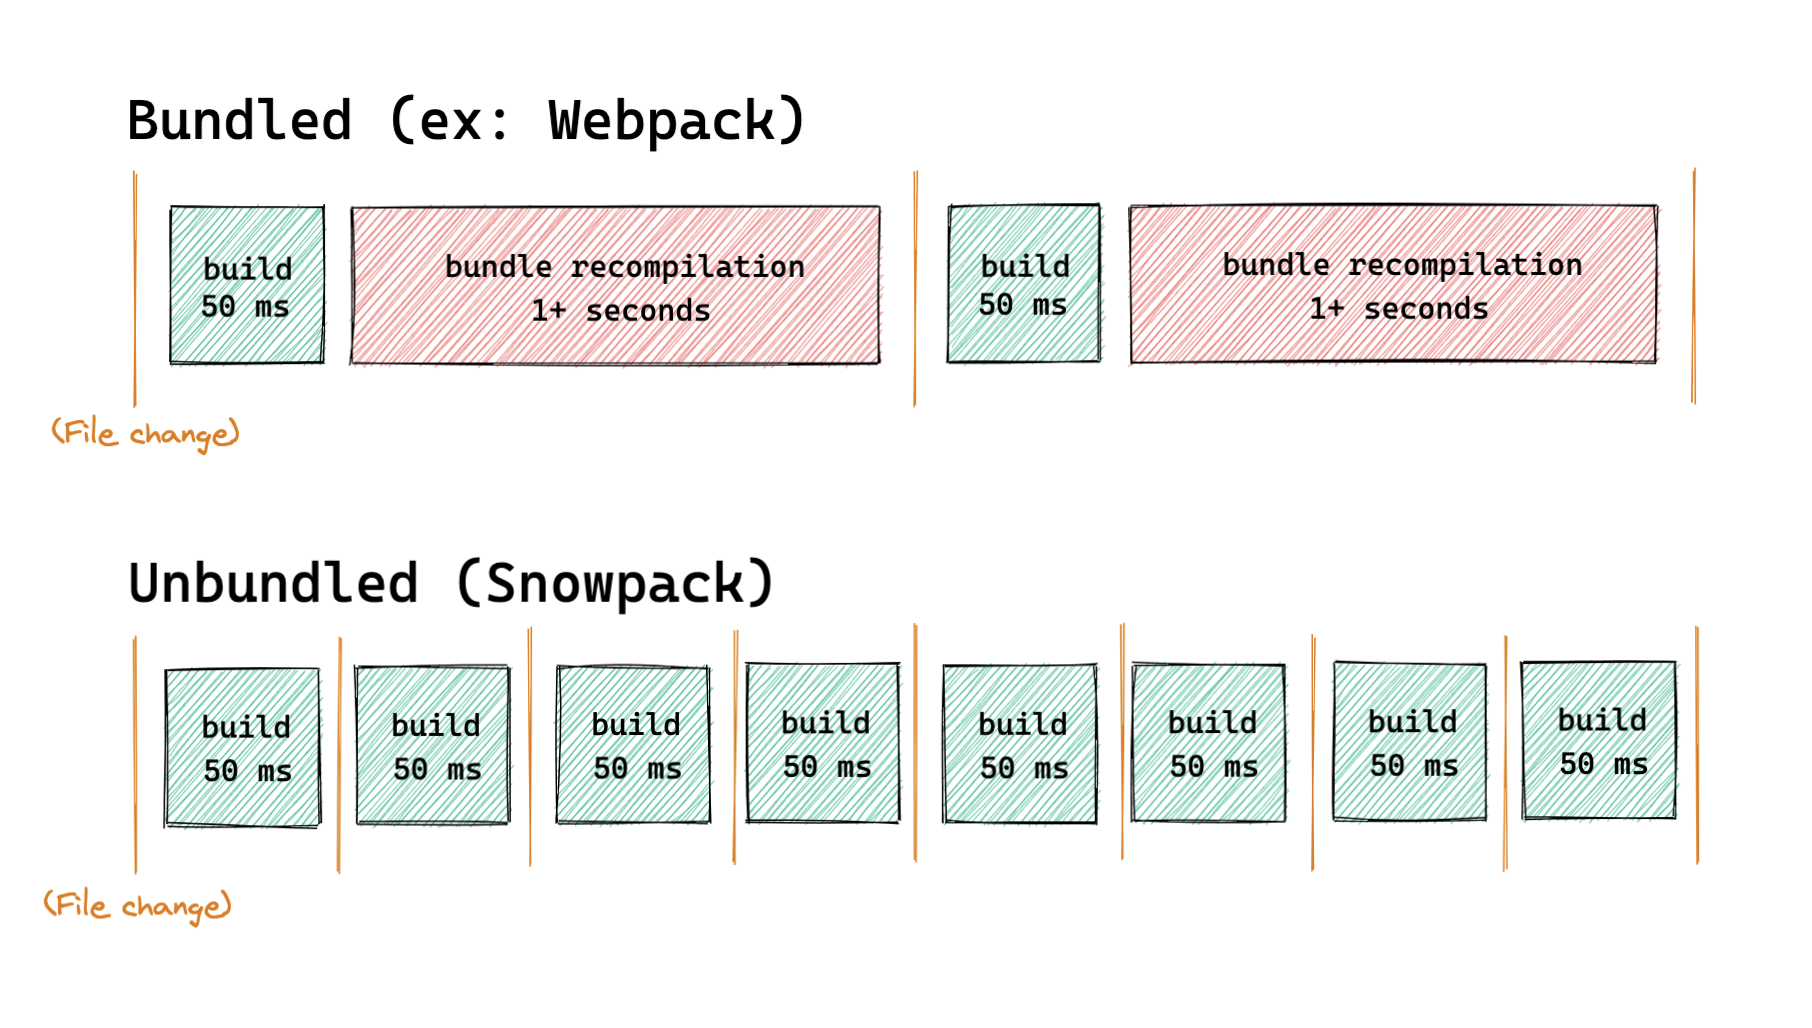
\includegraphics[scale=0.5]{Bundledvsunbundled}
   \caption{Gebundeld vs ongebundeld \autocite{snowpack-no-date}}
\end{figure}

Dit alles zou moeten resulteren in zeer snelle prestaties in vergelijking met module bundlers zoals Webpack. Wat echter niet betekent dat module bundlers voorbijgestreefd zijn. Sterker nog: ongebundelde build tools gebruiken ook module bundlers, de ene al meer dan de ander. Dit omdat de voordelen van Tree-shaking, een enkel uitvoerbestand en andere pluspunten van module bundlers nog steeds gelden. In hoofdstuk 3 en 4 zal hier dieper op ingegaan worden.

Voor de rest van deze proef zal de verzamelnaam “build tools” gebruikt worden om naar module bundlers en ongebundelde build tools te verwijzen. Module bundlers zijn namelijk ook tools die een webapplicatie helpen bouwen of builden, maar dan gebundeld. Waar mogelijk zal natuurlijk de meest specifieke term gebruikt worden.

\section{Keuze build tools}

In deze paragraaf zullen voorbeelden van build tools worden besproken. De keuze welke te bespreken gebeurt aan de hand van een requirement analyse. Die is vrij beknopt aangezien de requirements voor zowel module bundlers als ongebundelde build tools dezelfde zijn met uiteraard het verschil dat ze tot hun bepaalde categorie behoren.

\begin{itemize}
   \item Functionele requirements
   \begin{itemize}
     \item Een client side \gls{Javascript} webapplicatie kunnen bouwen
   \end{itemize}
   \item Niet-functionele requirements
   \begin{itemize}
     \item Typescript ondersteunen
     \item \gls{SASS} ondersteunen
     \item Statische bestanden ondersteunen
     \item Andere soorten bestanden kunnen importeren
   \end{itemize}
\end{itemize}

Hieruit volgt de long list voor module bundlers:
\begin{itemize}
\item Webpack
\item Parcel
\item Rollup
\item Fusebox
\item Browserify
\item Gulp
\item ESBuild
\item …
\end{itemize}

Module bundlers werken fundamenteel op dezelfde manier. Ze allemaal vergelijken is dus overbodig. Aangezien Webpack en Parcel het meest van elkaar verschillen zoals verder in dit hoofdstuk zal besproken worden en daarenboven twee van de meest populaire opties zijn \autocite{stateofjs-2020}, zullen zij de shortlist uitmaken. Rollup is ook een goede kandidaat maar komt al aan bod bij een ongebundelde build tool.

Ongebundelde build tools zijn relatief nieuw. Er zijn dus veel minder opties om uit te kiezen. Volgende opsomming fungeert dus zowel als long- en short list.

\begin{itemize}
\item Snowpack
\item Vite
\end{itemize}

\subsection{Webpack}

Webpack \autocite{webpack-2014} is de meest populaire module bundler in de wereld \autocite{stateofjs-2020}. Dit heeft veel te maken met het feit dat het één van de oudste is. Het is voorgeïnstalleerd in veel \gls{web frameworks} zoals create-react-app \autocite{facebook-2021} en Next.js \autocite{vercel-no-date}. Op deze manier wordt het door velen gebruikt zonder dat ze het weten. Webpack bevat een optionele ingebouwde ontwikkelserver die het opzetten van een lokale ontwikkelomgeving eenvoudiger maakt.

Webpack draait in een Node.js omgeving. Het kan zijn werk doen zonder enige configuratie, maar is zeer configureerbaar indien nodig. Het ondersteunt de hierboven besproken module types en meer. Omdat Webpack standaard alleen \gls{Javascript} en \gls{JSON} bestanden begrijpt, worden Loaders gebruikt om de verwerking van andere bestandstypen mogelijk te maken door ze om te zetten in geldige modules. Met behulp van Loaders kunnen andere typen modules of zelfs assets zoals afbeeldingen worden geïmporteerd en verwerkt door Webpack. Bovendien kan Webpack ook worden uitgebreid met plugins. Deze maken een brede waaier aan extra functionaliteit mogelijk, zoals verdere bundel optimalisatie. 

De functie van een module bundler is al besproken. Maar hoe bereikt Webpack dit? Wanneer een bestand afhankelijk is van een ander in een project, ziet Webpack dat en zet het in zijn dependency graph.

\begin{figure}[h]
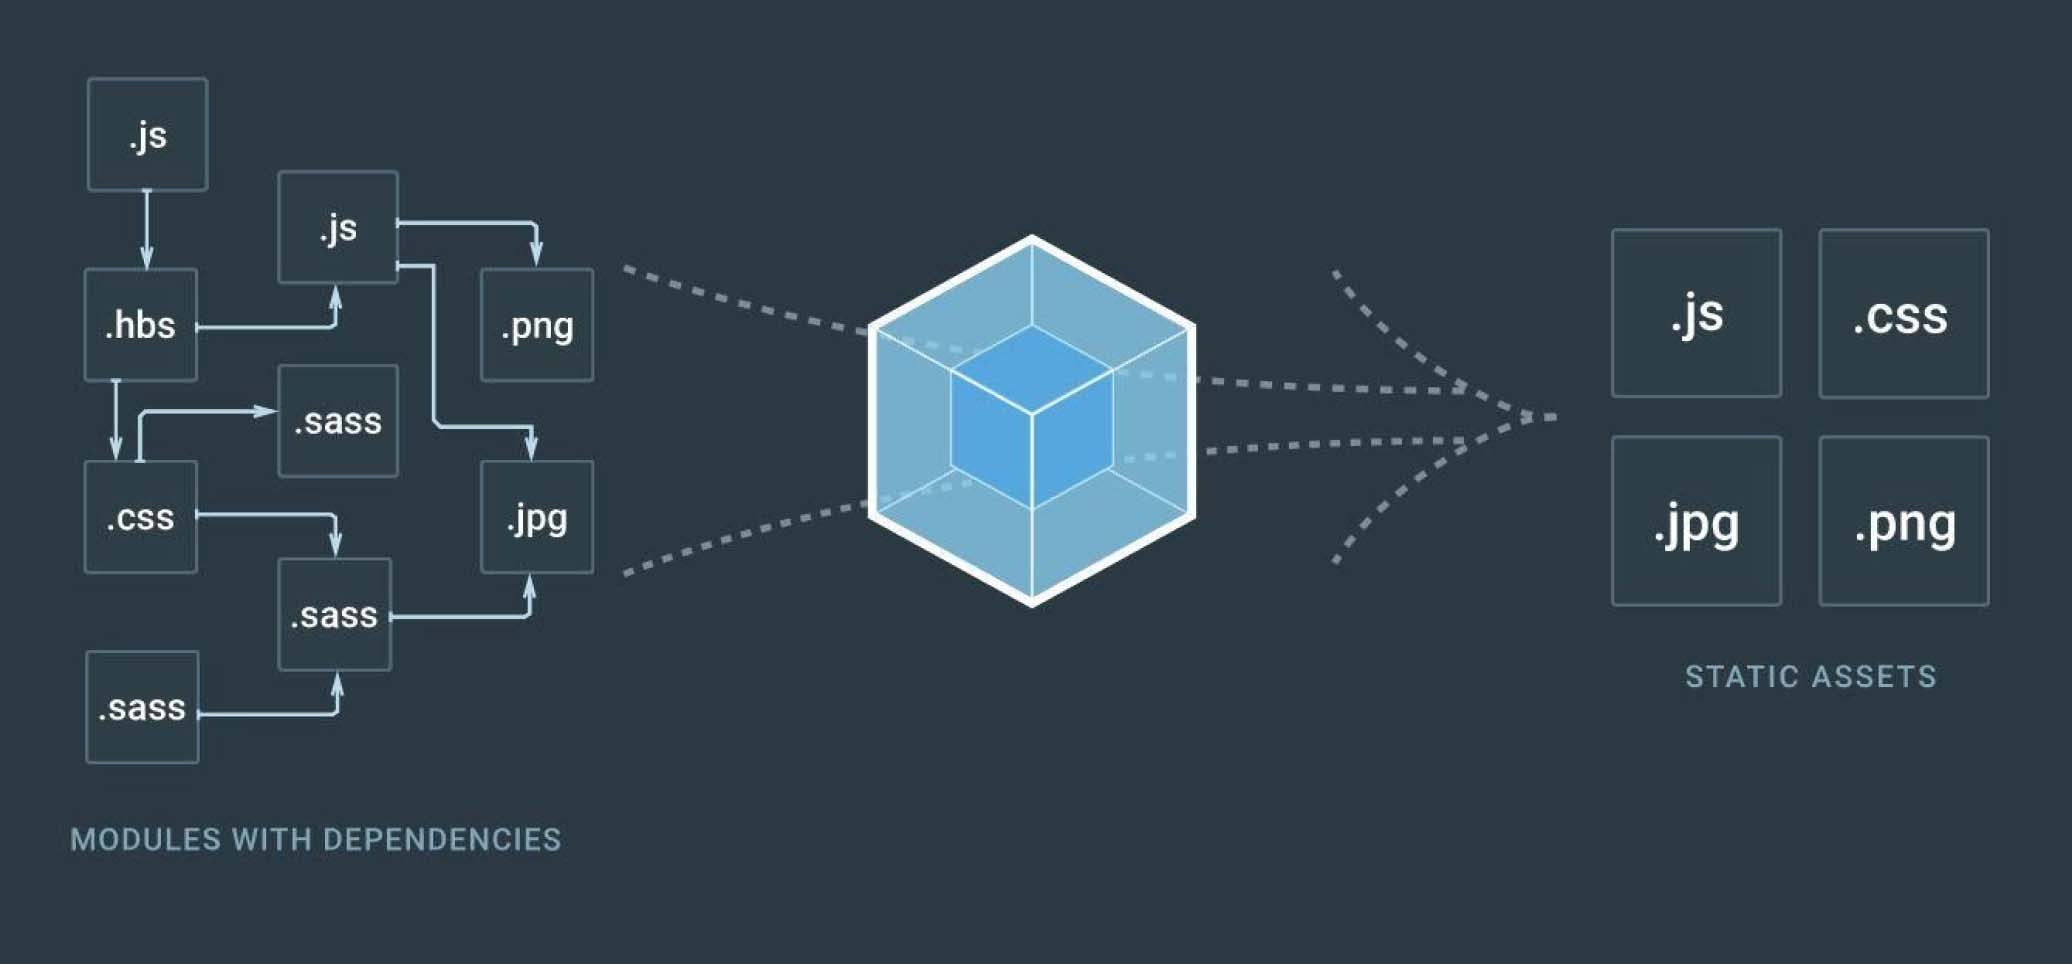
\includegraphics[scale=0.9]{Webpack}
   \caption{Essentiële functie module bundler \autocite{webpack-no-date}}
\end{figure}

Deze graaf wordt recursief opgebouwd. Wanneer het tijd is om de applicatie te bouwen, gebruikt het de dependency graph om alle bestanden samen te voegen tot één uitvoerbestand dat dan naar de browser wordt verzonden. Module bundlers, en dus ook Webpack, doen dit zowel in ontwikkeling als in productie. Met het belangrijk verschil dat bundelen in ontwikkelingsmodus iets anders is dan in productie. In ontwikkeling wordt bijvoorbeeld niet aan minificatie gedaan omdat het debuggen van een applicatie zo veel moeilijker zou zijn.

\subsection{Parcel}

Parcel \autocite{parcel-2020} is een andere module bundler. Het draait echter niet in een Node.js omgeving, in plaats daarvan gebruikt het een compiler die geschreven is in RUST. RUST is een gecompileerde programmeertaal. Zonder al te veel in detail te treden, betekent dit dat RUST code direct naar machinecode wordt gecompileerd, wat resulteert in snellere prestaties. De Javascript interpreter, en dus een hele stap, wordt hiermee overgeslagen. Parcel doet veel van dezelfde dingen die Webpack doet zonder enige configuratie. Toen het werd uitgebracht, was het belangrijkste kenmerk dat het geen configuratiebestand nodig had en Webpack wel. Nu kan Webpack echter ook zijn werk doen zonder een configuratiebestand. Hoewel een no-configuratie aanpak geweldig is voor kleinere projecten, kan het voor grotere applicaties niet haalbaar zijn.

\subsection{Snowpack}

Snowpack \autocite{snowpack-2019} is het eerste voorbeeld van een ongebundelde build tool. Het is momenteel de meest populaire in zijn categorie \autocite{stateofjs-2020}. Het pakt uit met de slogan ‘The faster build tool’. Of dat effectief waar is, zal in de volgende hoofdstukken besproken worden. Het grootste pluspunt van Parcel is dat die zijn doel probeert te bereiken met zo min mogelijk configuratie. Deze filosophie volgt Snowpack niet. Een configuratie bestand is vereist en kan al snel aanzienlijke grootte bereiken.

Zoals hierboven vermeldt, gebruikt een build tool vaak toch een module bundler in productie. Bij Snowpack is dit echter optioneel. Standaard is de productie build die Snowpack aanmaakt dus ook ongebundeld, iets waar enkel moderne browsers mee overweg kunnen. De configuratie kan wel aangepast worden om gebruik te maken van Webpack of Rollup zodat dat laatste geen probleem meer vormt. Voor dit onderzoek voegen we zo’n module bundler niet toe aan Snowpack. Bij de volgende build tool die aan bod komt, Vite, is het geen optie om de module bundler in productie weg te laten. Snowpack zal dus de volledig ongebundelde applicatie representeren, terwijl Vite hetzelfde zal doen voor de half-ongebundelde.

\subsection{Vite}
Vite \autocite{vite-2020} is de jongste build tool die in deze studie aan bod komt \autocite{vite-2020B}. Het combineert een ongebundelde ontwikkelingsomgeving met een gebundelde in productie. Voor dit laatste gebruikt het Rollup \autocite{vite-no-date}, een alternatief aan Webpack. Hoewel het ook een configuratiebestand bevat, is die veel minder groot en ingewikkeld dan Snowpack. 

Rollup is een module bundler die aan bod kwam in die categorie zijn long-list. Het focust vooral op het vertalen van ESModules naar andere soorten die wel ondersteund worden door het doelplatform. Hoewel Javascript nu eigen type module ondersteunt (ESM), is ze is alleen geïmplementeerd in moderne browsers en nog niet afgerond in Node.js. Rollup zorgt ervoor dat code geschreven kan worden met behulp van het nieuwe module-systeem, en zal dat dan vertalen naar de bestaande ondersteunde formaten, zoals CommonJS modules, IIFE’s, … . Rollup is niet optioneel bij Vite. Ze werken nauw samen om het beste van beide werelden te combineren. Wat dit alles betekent voor de eindgebruiker, volgt later.

Zoals de naam Vite doet vermoeden, beweren de makers ervan bliksemsnelle opstart- en buildtijden in vergelijking met de competitie.


In de twee volgende hoofdstukken zullen de besproken build tools getest en vergeleken worden. Eerst bij het opzetten van een nieuw project en daarna bij het omvormen van een bestaand. Elk hoofdstuk bevat een eigen conclusie, als laatste volgt de algemene.


\chapter{Nieuw project}

De traditionele methodologie is in deze proef opgedeeld in twee hoofdstukken. In de stand van zaken werden de verschillende te vergelijken build tools toegelicht. Deze zullen in de twee hoofdstukken naast elkaar gelegd en gequoteerd worden.
Eerst zal gekeken worden hoe ze verschillen bij het opzetten van een nieuw project. Daarna trachten we een bestaand project dat met Webpack opgezet is, om te vormen naar een van de andere opties. Elk hoofdstuk wordt afgesloten met een eigen besluit. Tot slot volgt in het laatste hoofdstuk een algemene, samenvattende conclusie.

Build tools hebben een enkel doel: een werkende webapplicatie afleveren. Hoe snel ze dat kunnen is de belangrijkste vergelijkende factor. Hieronder staan de twee factoren waar het meest rekening mee gehouden zal worden. Daarnaast zullen meer subjectieve factoren, zoals de gemakkelijkheid om ze werkende te krijgen, aan bod komen.

\begin{itemize}
   \item Snelheid creatie uitvoer voor productie
   \item Opstartsnelheid ontwikkelings server
\end{itemize}

Alle metingen werden gedaan op een M1 MacBook Pro en zijn reproduceerbaar aan de hand van deze repository \autocite{vansteenkiste-2021A}. De snelheidsmetingen werden gedaan aan de hand van een schermopname waardoor achteraf de snelheid accuraat kon waargenomen worden zonder ruimte voor menselijke fouten. Alle metingen werden driemaal uitgevoerd, met het verwijderen van cache bestanden waar mogelijk.

\section{Webpack}
Een nieuw project opzetten met Webpack kan op verschillende manieren: zelf een project opzetten en de configuratie volledig manueel schrijven of gebruik maken van een framework waarin het al geconfigureerd voor ons is. Aangezien niet velen het eerste pad bewandelen, zullen we gebruik maken van de meest populaire manier om een React project op te zetten. Create-react-app of CRA is een minimale framework gemaakt door de makers van React zelf om gemakkelijk een React omgeving op te zetten. Het is één van de vele frameworks die Webpack als module bundler gebruikt. Om te beginnen, voeren we volgende commando’s uit.

\lstinputlisting[language=bash]{codeSnippets/craCreate.txt}

Bovenstaande code maakt een project aan met create-react-app. Daarna ziet ons project er als volgt uit. Merk op dat er geen configuratie bestand voor Webpack is.

\begin{figure}[h]
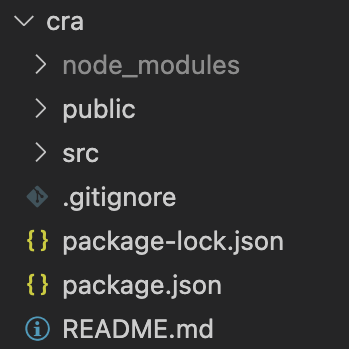
\includegraphics{fileStructureInitCRA}
   \centering
   \caption{Bestandsstructuur nieuw CRA project}
\end{figure}

Alles wat in de public map staat, zijn statische assets. Deze zullen via een url bereikbaar zijn. Als we kijken in het index.html bestand, merken we op dat er geen enkele script-tag aanwezig is. Hierover later meer.
In de src map staat alles wat door Webpack zal gebundeld worden. Standaard worden er CSS bestanden aangemaakt voor styling en een logo in svg formaat. Dit wordt gedaan om aan te tonen dat we deze assets gewoon in de Javascript code kunnen importeren, de bundler kan hiermee overweg.

\lstinputlisting[language=Javascript]{codeSnippets/importCSS.js}

In het package.json bestand staat er allemaal info over dit project. In het dependencies gedeelte staan alle externe packages die dit project gebruikt. Nieuwe packages worden gedownload aan de hand van Node Package Manager of NPM. Bij de dependencies staat een package genaamd “react-scripts”.
React-scripts \autocite{facebook-2018} is een package gemaakt door de makers van React en is de motor achter CRA.
Wat voor dit onderzoek relevant is, is dat het de Webpack.config bevat. Dit bestand bestaat uit maar liefst 700+ lijnen code \autocite{facebook-2021}. Nu is de reden dat we CRA gebruiken en niet van nul beginnen, duidelijk.

De volgende stap is om het project lokaal op te starten. React-scripts gebruikt de ingebouwde ontwikkelingsserver van Webpack. Na het uitvoeren van volgend commando, wordt die server opgestart en opent de webapplicatie in een browser.

\lstinputlisting[language=bash]{codeSnippets/craStart.txt}

\begin{table}[h]
   \centering
   \begin{tabular}{lr}
   \textbf{Grootte project (MB)} & 0,037 \\
   \textbf{Grootte node\_modules (MB)} & 214,1 \\
   \textbf{Grootte uitvoer (MB)} & 0,514 \\
   \textbf{Snelheid creatie uitvoer (s)} & 3,67 \\
   \textbf{} & 5 \\
   \textbf{} & 3 \\
   \textbf{} & 3 \\
   \textbf{Snelheid opstarten ontwikkelings server (s)} & 2,67 \\
   \textbf{} & 4 \\
   \textbf{} & 2 \\
   \textbf{} & 2
   \end{tabular}
   \caption{Overzicht nieuw project met Webpack}
   \end{table}

\section{Parcel}
Bij Webpack gebruikten we een framework om het vele configuratie werk te omzeilen. Bij Parcel is dit niet nodig. Zoals in de literatuurstudie vermeld werkt Parcel op een gelijkaardige manier als Webpack, maar dan met zo min mogelijk configuratie. Om een nieuw project op te zetten, gaan we dus geen framework gebruiken.

Maak een nieuwe map aan waar het project zal leven. Aangezien we van nul beginnen, moeten de bestanden uit figuur 3.2 zelf aangemaakt worden.

\begin{figure}[h]
   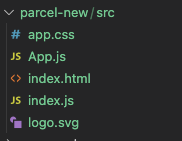
\includegraphics{parcelNew}
       \centering
       \caption{Aan te maken bestanden voor nieuw Parcel project}
   \end{figure}

Hierna moeten er nog enkele packages geïnstalleerd worden, namelijk: React, React-DOM en natuurlijk Parcel. In de package.json moet er ook nog meegegeven worden waar de index.html zich bevindt. Merk op dat er geen apart configuratiebestand voor Parcel is. Nu kan het project opgestart worden met hetzelfde commando als bij Webpack.

 Merk op dat er geen public map aanwezig is zoals in CRA. Er is momenteel geen map waar statische bestanden kunnen leven. Als dit een vereiste is, heeft Parcel een plugin nodig. Gelukkig is die gemakkelijk te installeren.

\section{Snowpack}
Voor Snowpack gaan we net zoals bij Parcel te werk zonder framework. In tegenstelling tot Parcel heeft het Snowpack team al een speciaal react-template gemaakt met een kant en klaar commando om het te initialiseren. Zelf de bestanden aanmaken en dependencies toevoegen is dus niet nodig.

\lstinputlisting[language=bash]{codeSnippets/snowpackNew.txt}
\begin{figure}[h]
   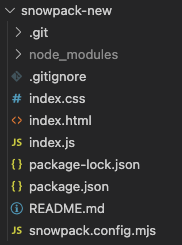
\includegraphics{snowpackNew}
       \centering
       \caption[Aangemaakte bestanden door Snowpack commando]{Aangemaakte bestanden door commado}
   \end{figure}

Deze structuur is identiek aan die van CRA. In tegenstelling tot Parcel is een public map al geconfigureerd voor statische bestanden, zoals afbeeldingen. Een configuratiebestand voor Snowpack is ook aangemaakt. Hierin staan al 25 lijnen configuratie voor ons geschreven. Meer dan Parcel maar aanzienlijk minder dan CRA. Merk op dat sommige bestanden nu de extensie .jsx in plaats van .js hebben. Dit komt doordat Snowpack geen JSX tolereert in .js bestanden. JSX is wat een React component retourneert i.e elk React component moet een .jsx extensie hebben. Geen probleem bij een nieuw project maar bij een oud kan het nodig zijn om vele bestanden van extensie te veranderen, zie later.

Zoals in de literatuurstudie vermeld, is Snowpack geen module bundler aangezien het de verschillende bestanden in een project niet bundelt. In productie kan dat optioneel nog gedaan worden door Webpack of Rollup maar dat is niet standaard. In ontwikkelings heeft dit het grote voordeel dat de bundel niet telkens opnieuw opgebouwd moet worden als een bestand veranderd.

\section{Vite}
Vite is nog een voorbeeld van een ongebundelde build tool, net zoals Snowpack. Een nieuw project opzetten is heel gemakkelijk aan de hand van een simpel commando dat ze voorzien hebben, net zoals Snowpack.

\lstinputlisting[language=bash]{codeSnippets/viteNew.txt}

\begin{figure}[h]
   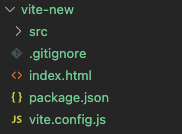
\includegraphics{viteNew}
       \centering
       \caption[Aangemaakte bestanden door Vite commando]{Aangemaakte bestanden door commado}
   \end{figure}

Er is een klein config bestand aanwezig van 7 lijnen code waar de react plugin is geïnitialiseerd. Voor de rest ziet het project in grote lijnen er uit als dat van Snowpack. Er is geen public map aanwezig maar dat kan aangemaakt worden en wordt automatisch geconfigureerd.


\section{Conclusie}
Al de build tools hebben niet gezweet bij het opzetten van een nieuw project, wat maar normaal is. Voor Webpack is er gebruik gemaakt van een framework, CRA, omdat het configuratie werk anders te veel zou zijn. Ook al is het een nieuw project en dus relatief klein, toch kunnen we al verschillen waarnemen tussen de vier kandidaten.

Op onderstaande figuur zien we al een trend verschijnen die doorheen deze conclusie zal gelden: Webpack is aanzienlijk trager dan de competitie, ondanks dat Snowpack niet bundelt, is het toch even traag of trager dan Parcel. Die laatste zijn Rust compiler, zie literatuurstudie, zal zijn vruchten afwerpen. De drie balkjes die ontbreken bij Vite en het ene bij Parcel zijn geen fout: zij waren gewoon sneller dan een volledige seconde.

\begin{figure}[h]
   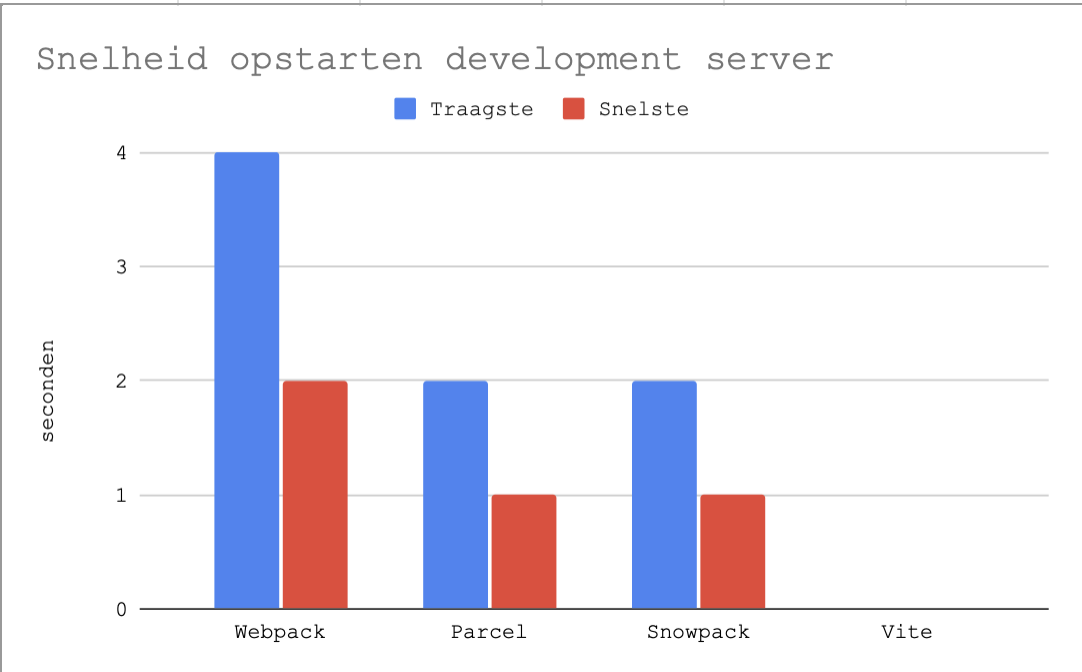
\includegraphics[scale=0.6]{conslusieNieuwDev}
       \centering
       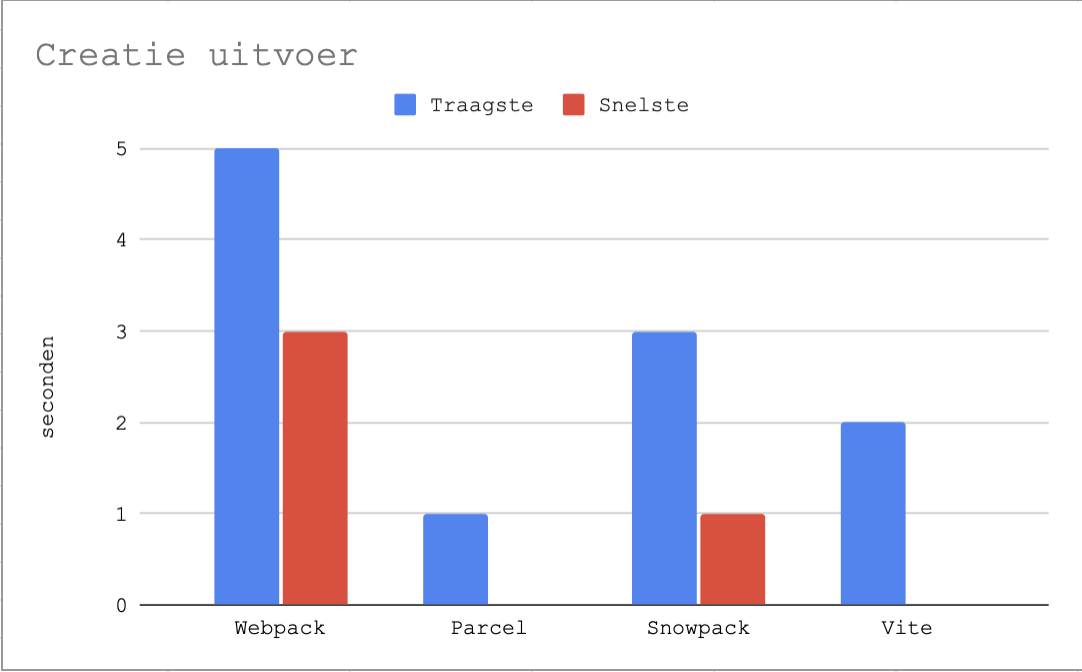
\includegraphics[scale=0.6]{conclusieNieuwUitvoer}
       \centering
       \caption{Resultaten nieuw project}
   \end{figure}


De developer experience was voor al de build tools zo goed als dezelfde bij het opzetten van dit nieuw project. De conclusie kunnen we daarop dus niet baseren. Maar de data hierboven is duidelijk genoeg: bij het opzetten van een project is Vite de beste optie. Het gebruikt het beste van beide werelden: ongebundelde code in ontwikkeling en gebundelde code in productie. De andere opties hebben niet direct een afknapper, maar de snelheid van Vite valt niet te negeren.

\chapter{Bestaand project}

In het vorig hoofdstuk, werden nieuwe projecten opgezet met de respectievelijke build tools. In dit hoofdstuk worden bestaande projecten, opgezet met Webpack, omgevormd zodat ze gebruik maken van de andere opties. Per project wordt eerst wat toelichting gegeven en vervolgens per build tool wat er nodig is om ze werkende te krijgen.

Er is dus nood aan bestaande projecten om de build tools te kunnen testen. Gelukkig zijn er online genoeg open-source voorbeelden hiervan te vinden. Drie projecten werden gekozen aan de hand van hun grootte en technologieën die ze gebruiken. Eén eigenschap hebben ze allemaal gemeen: het zijn Javascript projecten die React als UI library gebruiken. De reden dat geen projecten gekozen werden met andere UI libraries zoals Vue, is omdat React veel meer gebruikt wordt, ook door de co-promotor. Desondanks zijn de gekozen projecten ook representatief voor de andere UI libraries aangezien ze uiteindelijk allemaal Javascript zijn.

\section{Mortage}
Het eerste project dat we gaan omvormen is de Mortage Overpayment Calculator \autocite{houghton-2019}.
Het is een zeer simpel en klein project van 17 KB groot dat is opgezet met CRA.
Daarnaast maakt het nog gebruik van andere open-source packages die verzameld worden in de nodemodules map.
Die map is 214 MB groot.

Mortage is een ideaal project om mee te starten aangezien het geen speciale technologieën gebruikt. CSS voor stijl, wat de browser begrijpt zonder enige omvorming en voor de rest Javascript en HTML. Normaal zouden we dus niet in de problemen mogen komen. Een potentiële moeilijkheid wat dit project ook vermijdt is een map voor statische bestanden.

\begin{figure}[h]
   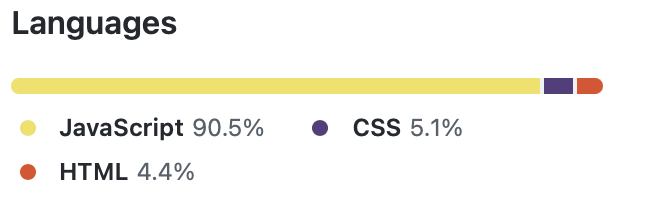
\includegraphics{Mortage_languages}
       \centering
       \caption{Overzicht gebruikte technologieën van het Mortage project}
 \end{figure}

\subsection{Parcel}
Zoals in de literatuurstudie vermeld, probeert Parcel hetzelfde als Webpack te bereiken maar met veel minder tot geen configuratie. Die bewering zal nu nagegaan worden. Mortage is opgezet met CRA en gebruikt dus het react-scripts package die onder andere alle Webpack configuratie op zich neemt. Om Webpack in te ruilen voor Parcel moeten we dus eerst react-scripts bij het grofvuil zetten. Het package.json bestand bevat alle info over een project: de naam, versie, welke andere packages het gebruikt, hoe het wordt opgestart en nog veel meer. Ook Mortage heeft zo’n bestand en dat ziet er als volgt uit:

\lstinputlisting[language=Javascript]{codeSnippets/packageMortage.json}

In het gedeelte “scripts” staan de verschillende commando’s. Het start en build commando starten het project in ontwikkelings- en productiemodus respectievelijk op. Beide voeren op hun beurt een commando van react-scripts uit. Dit gaat dus vervangen moeten worden. In de documentatie van Parcel valt te lezen dat we die commando’s moeten vervangen met de volgende:

\lstinputlisting[language=Javascript]{codeSnippets/scriptsParcelMortage.json}

Vervolgens moet het index.html bestand aangepast worden. Voor de wijzigingen zag het er als volgt uit:

\lstinputlisting[language=HTML]{codeSnippets/mortageIndex.html}

Merk op dat er nergens een verwijzing is naar een Javascript bestand. React-scripts voegt dat automatisch toe bij het bouwen van het project. Parcel doet dat niet dus er moet nog een expliciete verwijzing komen.

\lstinputlisting[language=HTML]{codeSnippets/mortageIndexScript.html}

Nu moet Parcel uiteraard nog gedownload worden. Nadien werkt het project.

\subsection{Snowpack}
Snowpack is een ontwikkelings build tool zoals uitgelegd in de literatuurstudie. Wat dat betekent in de werkelijkheid volgt later. Eerst kijken we hoe Mortage kan omgevormd worden van Webpack naar Snowpack.

Bij Parcel lag de focus op zo weinig mogelijk configuratie, niet bij Snowpack. Snowpack is veel moeilijker te configureren dan Parcel en Vite en voelt in dat opzicht aan als Webpack. We ondernemen dezelfde stappen als hierboven om react-scripts te verwijderen en die te vervangen door de nieuwe commando’s. Daarna voegen we Snowpack toe samen met twee andere plugins voor React. We doen net dezelfde wijzigingen aan index.html, voegen een configuratie bestand toe en proberen de app te runnen. Een foutmelding verschijnt. Om die te kunnen begrijpen, is er eerst wat meer uitleg nodig.

Een React component retourneert JSX. JSX is, zonder te veel in details te gaan, een extensie bovenop Javascript die een manier biedt om de weergave van componenten te structureren en lijkt heel hard op HTML. Het belangrijke om hiervan mee te nemen is dat het een Javascript extensie is. In CRA en sommige andere frameworks is het mogelijk om JSX in een bestand te schrijven met de standaard Javascript extensie .js . Snowpack ondersteunt dit niet. Als een bestand JSX bevat, moet die de extensie .jsx krijgen. Dus moeten we alle bestanden die JSX gebruiken van bestandsextensie veranderen. Hierna werkt de app naar behoren.

\subsubsection{Vite}

Vite combineert het beste van de twee voorgaande build tools. Het is een ontwikkelings build tool in ontwikkelingsmodus en een module bundler in productie, en dat alles zonder al te veel configuratie. Om Mortage op te zetten met Vite overlopen we stappen die eerder al aan bod kwamen: react-scripts verwijderen, index.html voorzien van een script-tag en package.json naar de nieuwe commando’s aanpassen en Vite zelf installeren. Net zoals Snowpack ondersteunt Vite geen JSX in een .js bestand en is er een plugin voor React. In tegenstelling tot Snowpack is de plugin niet nodig om het project werkend te krijgen. Na het aanpassen van de bestandsextensies en eventueel downloaden van de plugin, kan dit project zonder problemen opgestart worden.

\subsection{Todoist}

Todoist \autocite{hadwen-2021} is een simpele to-do webapplicatie. Een gebruiker kan taken toevoegen die nog moeten gedaan worden en aanduiden wanneer die voltooid zijn. Het is een groter project dan Mortage met een grootte van 106KB en 377MB nodemodules maar kan nog steeds beschouwd worden als een kleine tot medium grootte app. Het heeft een database nodig om de taken te kunnen opslaan en zoals hieronder te zien is, gebruikt het een andere taal voor stijl: SCSS. SCSS is een superset of uitbreiding van gewone CSS. Aangezien een webbrowser die uitbreiding niet ondersteunt, moet het SCSS bestand omgevormd worden naar gewone CSS wanneer de applicatie start. Dit kan eventueel tot extra configuratie leiden bij het instellen van een nieuwe build tool.

\begin{figure}[h]
   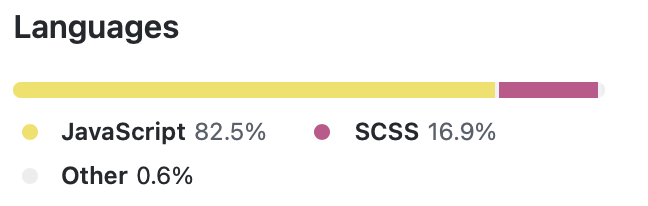
\includegraphics{Todoist_languages}
       \centering
       \caption{Overzicht gebruikte technologieën van het Todoist project}
   \end{figure}

\subsubsection{Parcel}

Om dit project om te vormen naar Parcel worden eerst dezelfde stappen overlopen als in het vorige Parcel project. Er zijn twee mogelijke extra struikelblokken bij Todoist: het gebruik van SCSS en statische bestanden. Het eerste overkomt Parcel met glans: we moeten niets zelf configureren. De eerste keer dat Todoist wordt gestart, detecteert Parcel dat er SCCS aanwezig is en download de bijhorende plugin. Het tweede probleem vereist ook een plugin en daarenboven nog wat configuratie. In de package.json duiden we met enkele lijnen aan waar het mapje met statische bestanden zich bevindt. Nadien moeten de verwijzingen naar de afbeeldingen nog veranderd worden naar de nieuwe locatie. Hierna is ook dit project bijna klaar voor gebruik. Enkel nog het configuratie bestand voor de database moet nog aangepast worden.

\subsubsection{Snowpack}

Ook hier zijn de stappen gelijkaardig aan het vorig project. Na die te doorlopen volgen de twee potentiële moeilijkheden. In het vorig deel over Snowpack werd al vermeld dat statistische bestanden ondersteund worden zonder extra plugin. Het tweede probleem, SCSS, kan eveneens opgelost worden door een plugin. In tegenstelling tot Parcel, moet die wel manueel toegevoegd worden.

\subsubsection{Vite}

Voor Vite kunnen we heel kort blijven. Na het uitvoeren van dezelfde stappen als vorig project, werkt alles. Zowel statische bestanden als SCCS zijn ondersteunt zonder extra plugins of configuratie.

\subsection{Bar}
Als laatste nemen we het grootste en meest complexe project van deze studie onder de loep. De BarApp \autocite{vansteenkiste-2021} is ontworpen om barlijsten bij te houden zonder zelf rekening te houden met de effectieve betaling. In vergelijking met de voorgaande projecten is het veel groter: 27MB voor het project zelf en dan nog eens 442MB voor de nodemodules. SCCS valt weg als moeilijkheid en wordt vervangen door twee nieuwe: TypeScript en Tailwind CSS.

\begin{figure}[h]
   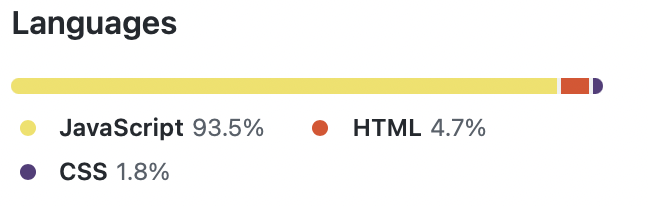
\includegraphics{Barapp_languages}
       \centering
       \caption{Overzicht gebruikte technologieën van het BarApp project}
 \end{figure}

TypeScript is net als SCCS een superset of uitbreiding. Deze keer niet van CSS maar van Javascript. De browser begrijpt geen TypeScript dus moet het eerst vertaald worden naar normale Javascript. De build tools zijn hier verantwoordelijk voor.

De tweede moeilijkheid, Tailwind CSS, staat niet in het gebruikte-talen-overzicht van hierboven. Toch is het iets waar we rekening mee moeten houden. Het is een collectie van allemaal CSS klassen die de gebruiker direct in een JSX element kan gebruiken. Tailwind zelf bevat dus hele grote CSS bestanden om die klassen allemaal te definiëren. Aangezien we enkel de klassen willen behouden die effectief gebruikt worden in het project, worden de ongebruikte gewist bij het bouwen van de applicatie voor productie. Hoewel dit alles geen taak is van de build tool zelf, kunnen er moeilijkheden optreden bij de configuratie.
  
\subsubsection{Parcel}

Nog maar eens overkomt Parcel de mogelijke struikelblokken met zo goed als geen configuratie. Het ondersteunt Typescript zonder iets extra te moeten doen. Naast de standaard configuratie van Tailwind zelf, is er niets anders nodig om het werkend te krijgen. Na het overlopen van de stappen van de vorige Parcel projecten, met in het bijzonder de stap voor statische bestanden, is ook deze applicatie bijna klaar voor gebruik. Voor het laatste detail nemen we nog een kijkje naar de index.html. Aangezien CRA op een andere manier verwijst naar de afbeeldingen die hier staan, moeten de href attributen aangepast worden.

\subsubsection{Snowpack}
Om al een tipje van de sluier op te lichten: dit project was veel lastiger om op te zetten met Snowpack dan met de andere twee opties. Eerst het goede nieuws: Typescript is ook ondersteund zonder extra configuratie. Daar stopt de vreugde al. De overige problemen worden door hun complexiteit in paragrafen onderverdeeld.

Voor Tailwind CSS valt het nog wel mee. Naast dezelfde configuratie en installatie stappen die moeten doorlopen worden als bij Parcel (en Vite), moet er nog een plugin geïnstalleerd worden voor Snowpack zelf. Hierna moet die zijn configuratie bestand aangepast worden zodat de plugin kan werken. Dat doen we door op twee verschillende plaatsen een lijn code toe te voegen.

Zoals in de literatuurstudie uitgelegd, ondersteunen moderne browsers enkel ESM. Aangezien Snowpack een ongebundelde build tool is, stuurt het de bestanden van het project naar de browser zonder ze te bundelen.

\begin{figure}[h]
   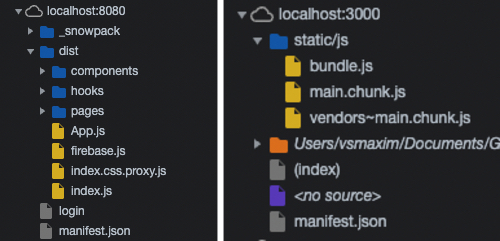
\includegraphics{bundledVSUnbundledFiles}
       \centering
       \caption{Bestandsstructuur ongebundeld vs gebundeld}
 \end{figure}

Merk op dat bij de ongebundelde versie van dit project, de bestandsstructuur dezelfde is als hoe we het project maken. Een bundler zoals Webpack, steekt alle bestanden die naar elkaar verwijzen samen in één bestand dat dan naar de browser gestuurd wordt. ongebundelde build tools zoals Snowpack laten de bestandsstructuur met rust omdat ze vertrouwen op het feit dat moderne browsers ESM ondersteunen. Dus zolang er in het project enkel ESM wordt gebruikt, is er geen probleem. Jammer genoeg staat er in de App.jsx een require functie, een CommonJS module dus. Omdat Snowpack niets doet om dit te vertalen zal de CommonJS module manueel omgevormd moeten worden naar ESM. Gelukkig wordt die vertaling wel uitgevoerd voor de node-modules, want die bevatten ook vaak CommonJS.

Voor het volgend probleem, wordt het index.jsx bestand onder de loep genomen.

\lstinputlisting[language=Javascript]{codeSnippets/indexBar.js}

De aangeduide code vormt een probleem. De lijn process.env.NODE env === “production” wordt gebruikt om te kijken of de app in productie draait of lokaal, in ontwikkelingsmodus. Naast dit voorbeeld wordt deze methode vaak toegepast in dit en andere projecten. Het probleem is dat Snowpack het niet ondersteunt. Omdat dit voorbeeld niet cruciaal is, laten we het weg om Snowpack opgezet te krijgen. Jammer genoeg gebruikt deze app Workbox. Workbox is een Javascript bibliotheek die een PWA opzetten, gemakkelijker maakt. Een PWA is een webapplicatie die installeerbaar is op een Smartphone of computer. Het probleem is dat Workbox ook gebruikt maakt van bovenstaande methode. Als we deze bibliotheek nog steeds zouden willen gebruiken, zou dit alles ook moeten herschreven worden. Voorlopig gaan we verder zonder aangezien het veel tijd in beslag zou nemen. Op naar het laatste probleem.

React kan al even gebruikt worden zonder het te moeten importeren in een bestand. Dat wordt automatisch voor de developer gedaan. Jammer maar helaas: Snowpack ondersteunt dit niet. Aan elk Javascript bestand waar iets van de React methodes gebruikt wordt, moet een import statement toevoegen als volgt:

   \lstinputlisting[language=Javascript]{codeSnippets/importReact.js}

Na dit alles te overlopen, weliswaar zonder PWA-functionaliteit, werkt het project. Eindelijk.

\subsubsection{Vite}
Na de hele waslijst problemen die bij Snowpack opdoken, doet het deugd om weer met Vite aan de slag te mogen gaan. Van de struikelblokken die Snowpack tegenkwam, blijft voor Vite enkel nog het probleem van de CommonJS module over. Na die te herschrijven en dezelfde stappen te doorlopen als bij de vorige Vite secties, werkt dit project volledig, ook Workbox. Typescript is ondersteund zonder extra gedoe en voor Tailwind is de gebruikelijke installatie en configuratie nodig, geen extra plugin. Net zoals bij Parcel moeten de verwijzingen naar de afbeeldingen in de index.html bijgeschaafd worden.

\section{Conclusie}
Een bestaand project omvormen is het heel andere koek gepaard met andere overwegingen. In de methodologie is getracht projecten te kiezen met zoveel mogelijk uiteenlopende technologieën. Natuurlijk is lang niet alles aan bod gekomen. Een project kan bestaan uit talloze combinaties van verschillende, soms niche technologieën, packages of zelf geschreven bibliotheken. Wat in dit onderzoek geconcludeerd zal worden, is een overweging gebaseerd op de projecten die hier aan bod gekomen zijn. Het kan zijn dat voor een ander project, die keuze minder gemakkelijk of zelfs uitgesloten is door welke factor dan ook. Dat terzijde, de conclusie zal in het algemeen voor de meeste gelden aangezien veel voorkomende use-cases aan bod kwamen. Onderstaande resultaten zouden hoogstwaarschijnlijk nog kunnen bijgeschaafd worden door van elke build tool de configuratie te optimaliseren per project. Dit echter is niet het punt van deze studie. Welke build tool is in het algemeen de beste keuze, zonder uren de configuratie bij te schaven?

Op onderstaande figuur is te zien dat elke geteste build tool het beter doet dan Webpack en het verschil is vaak niet klein. Hoewel Snowpack ook aanzienlijk sneller is maar uit de methodologie bleek is dat de developer experience ver van optimaal is, zeker in vergelijking met de andere opties, kijk je beter elders bij het kiezen van een nieuwe build tool. Parcel en Vite daarentegen doen het heel goed op vlak van developer experience en snelheid. Parcel levert gebundelde code af, ook in ontwikkelingsmodus. Dit kan een voor- of nadeel zijn, afhangend hoe het bekeken wordt. Uit het vorig hoofdstuk blijkt dat Vite geen CommonJS ondersteunt, Parcel wel. Hoewel Parcel in sommige scenario’s net iets sneller weet te zijn dan Vite, wint die laatste toch in de meeste gevallen. Merk op dat ook bij de tweede grafiek, het balkje bij Vite ontbreekt. Dit is weer geen fout: Vite slaagt erin om zijn ontwikkelingsserver gemiddeld in sneller dan een seconde op te starten. Dat is indrukwekkend, zeker als dit naast de resultaten van de competitie gelegd wordt.

\begin{figure}[h]
   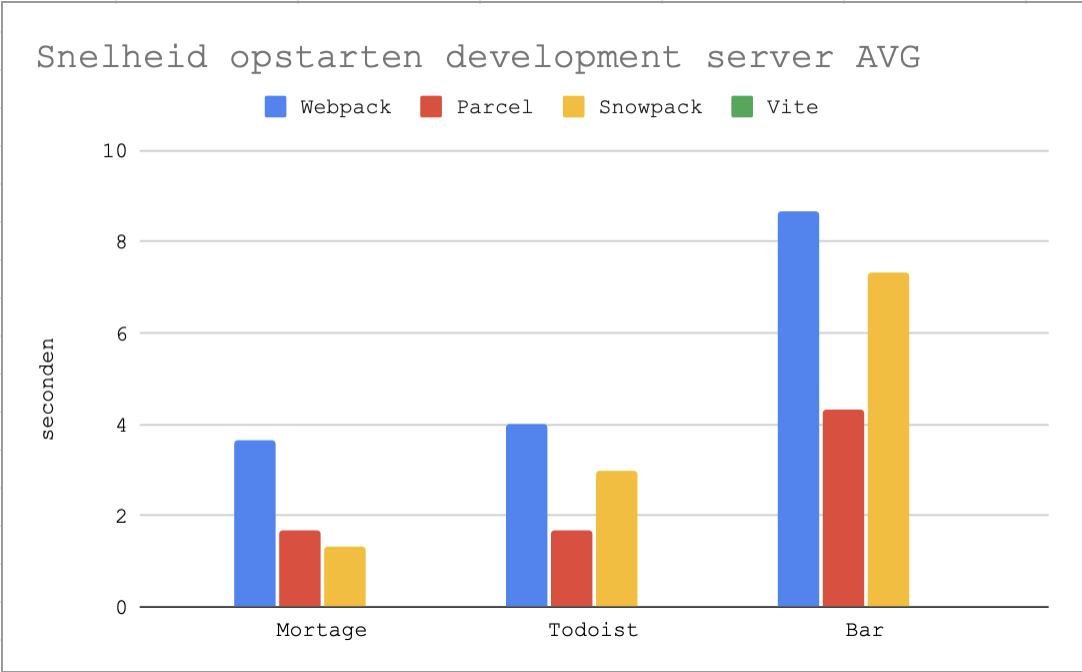
\includegraphics[scale=0.6]{conclusieBestaandDev}
       \centering
       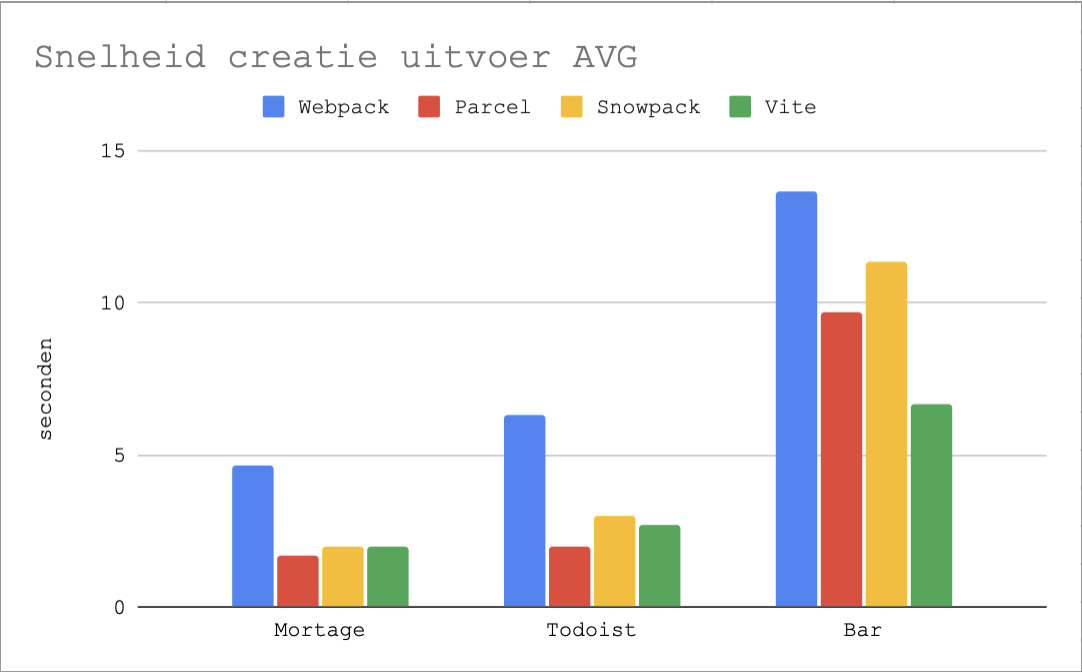
\includegraphics[scale=0.6]{conclusieBestaandUitvoer}
       \centering
       \caption{Resultaten bestaand project}
 \end{figure}
 


% Voeg hier je eigen hoofdstukken toe die de ``corpus'' van je bachelorproef
% vormen. De structuur en titels hangen af van je eigen onderzoek. Je kan bv.
% elke fase in je onderzoek in een apart hoofdstuk bespreken.

%\input{...}
%\input{...}
%...

\chapter{Conclusie}
\label{ch:conclusie}

In de twee vorige hoofdstukken werden de gekozen build tools op de proef gesteld aan de hand van drie open-source projecten en een van nul te beginnen. De verschillende stappen om ze werkende te krijgen werden overlopen, bij de een waren dat er al meer dan de ander. Bij elk van die twee hoofdstukken werd op het einde ook een aparte conclusie getrokken. Dit hoofdstuk dient als algemene conclusie. 

De hoofdvraag van deze proef, of Webpack nog steeds mag gezien worden als de koning der Javascript build tools, kan beantwoord worden met een duidelijke ‘nee’. Zelf binnen zijn eigen categorie van module bundlers, blijkt Parcel, in de meeste gevallen, een betere optie te zijn. Vite bewees dat de ongebundelde build tools de toekomst zijn. Module bundlers zijn hierdoor echter nog niet voorbijgestreefd. Zelfs wanneer browsers en Node.js ESModules volledig ondersteunen en alle open-source packages er volledig mee geschreven zijn, zullen de voordelen van module bundlers hun plaats in de Javascript wereld garanderen. Voor de nabije toekomst zullen module bundlers en ongebundelde build tools hand in hand moeten samenwerken om het beste van beide werelden samen te brengen. Vite lijkt dit het best te begrijpen. Het is dus wel duidelijk dat Vite de beste optie is voor zowel een nieuwe webapplicatie te ontwikkelen, als een bestaand een nieuwe, snellere en modernere motor te geven. 



%%=============================================================================
%% Bijlagen
%%=============================================================================

\appendix
\renewcommand{\chaptername}{Appendix}

%%---------- Onderzoeksvoorstel -----------------------------------------------

\chapter{Onderzoeksvoorstel}

Het onderwerp van deze bachelorproef is gebaseerd op een onderzoeksvoorstel dat vooraf werd beoordeeld door de promotor. Dat voorstel is opgenomen in deze bijlage.

% Verwijzing naar het bestand met de inhoud van het onderzoeksvoorstel
%---------- Inleiding ---------------------------------------------------------

\section{Introductie} % The \section*{} command stops section numbering
\label{sec:introductie}

A module bundler is one of the most essential technologies in modern web development. Nobody makes webapps with plain HTML, CSS and JS anymore. So the choice of which bundler to use is very important.
While Webpack is the most popular there are many others that claim to do the job better than it. Why is it still the king then I wonder. How does Webpack compare to its competitors? Are their claims true? If so, why is Webpack still the most popular? With this paper. 

Many developers give much thought about which framework to use, which back-end and so forth. The module bundler however often doesn't get that much thoutgh. This is because it's less attractive and in many frameworks comes pre-installed. But as your webapp can't run without it, I believe . In this paper, I want to demystify the module bundler and compare the most popular options. Not just in terms of speed and module size, but also its plugins, developer experience, ... .

Hier introduceer je werk. Je hoeft hier nog niet te technisch te gaan.

Je beschrijft zeker:

\begin{itemize}
  \item de probleemstelling en context
  \item de motivatie en relevantie voor het onderzoek
  \item de doelstelling en onderzoeksvraag/-vragen
\end{itemize}

%---------- Stand van zaken ---------------------------------------------------

\section{State-of-the-art}
\label{sec:state-of-the-art}

Much has already been written about module bundlers online. However many don't go in depth with the workings of it or stay very superficial. While they provide very useful information, I

Hier beschrijf je de \emph{state-of-the-art} rondom je gekozen onderzoeksdomein. Dit kan bijvoorbeeld een literatuurstudie zijn. Je mag de titel van deze sectie ook aanpassen (literatuurstudie, stand van zaken, enz.). Zijn er al gelijkaardige onderzoeken gevoerd? Wat concluderen ze? Wat is het verschil met jouw onderzoek? Wat is de relevantie met jouw onderzoek?

Verwijs bij elke introductie van een term of bewering over het domein naar de vakliteratuur, bijvoorbeeld~\autocite{Doll1954}! Denk zeker goed na welke werken je refereert en waarom.

% Voor literatuurverwijzingen zijn er twee belangrijke commando's:
% \autocite{KEY} => (Auteur, jaartal) Gebruik dit als de naam van de auteur
%   geen onderdeel is van de zin.
% \textcite{KEY} => Auteur (jaartal)  Gebruik dit als de auteursnaam wel een
%   functie heeft in de zin (bv. ``Uit onderzoek door Doll & Hill (1954) bleek
%   ...'')

Je mag gerust gebruik maken van subsecties in dit onderdeel.

%---------- Methodologie ------------------------------------------------------
\section{Methodologie}
\label{sec:methodologie}

Hier beschrijf je hoe je van plan bent het onderzoek te voeren. Welke onderzoekstechniek ga je toepassen om elk van je onderzoeksvragen te beantwoorden? Gebruik je hiervoor experimenten, vragenlijsten, simulaties? Je beschrijft ook al welke tools je denkt hiervoor te gebruiken of te ontwikkelen.

%---------- Verwachte resultaten ----------------------------------------------
\section{Verwachte resultaten}
\label{sec:verwachte_resultaten}

Hier beschrijf je welke resultaten je verwacht. Als je metingen en simulaties uitvoert, kan je hier al mock-ups maken van de grafieken samen met de verwachte conclusies. Benoem zeker al je assen en de stukken van de grafiek die je gaat gebruiken. Dit zorgt ervoor dat je concreet weet hoe je je data gaat moeten structureren.

%---------- Verwachte conclusies ----------------------------------------------
\section{Verwachte conclusies}
\label{sec:verwachte_conclusies}

Hier beschrijf je wat je verwacht uit je onderzoek, met de motivatie waarom. Het is \textbf{niet} erg indien uit je onderzoek andere resultaten en conclusies vloeien dan dat je hier beschrijft: het is dan juist interessant om te onderzoeken waarom jouw hypothesen niet overeenkomen met de resultaten.



%%---------- Andere bijlagen --------------------------------------------------
% TODO: Voeg hier eventuele andere bijlagen toe
%\input{...}

%%---------- Referentielijst --------------------------------------------------

\printbibliography[heading=bibintoc]

\end{document}
